%!TEX TS-program = xelatex
%!TEX encoding = UTF-8 Unicode
%!BIB TS-program = bibtex
% !TeX spellcheck = en_US
\documentclass[12pt]{article}
\usepackage[english]{babel}
\usepackage{url}
\usepackage[utf8x]{inputenc}
\usepackage{amsmath}
\usepackage{graphicx}
\graphicspath{{images/}}
\usepackage{parskip}
\usepackage{fancyhdr}
\usepackage{vmargin}
\usepackage{enumerate}
\usepackage[T1]{fontenc}
\usepackage{newpxtext,newpxmath}
\usepackage{booktabs}
\usepackage{siunitx}
\usepackage[version=4]{mhchem}
\usepackage{hyperref}
\usepackage{bm}
\setmarginsrb{3 cm}{2.5 cm}{3 cm}{2.5 cm}{1 cm}{1.5 cm}{1 cm}{1.5 cm}
\sisetup{inter-unit-product = \ensuremath{{}\cdot{}}}
\DeclareTextCommand{\nobreakspace}{T1}{\leavevmode\nobreak\ }
\newcommand{\ii}{{\mathrm{i}}}
\newcommand{\ee}{\mathrm{e}}

\title{Solid State Physics HW 1}								% Title
\author{XYZ}								% Author
\date{}											% Date

\makeatletter
\let\thetitle\@title
\let\theauthor\@author
\let\thedate\@date
\makeatother

\pagestyle{fancy}
\fancyhf{}
\rhead{\theauthor}
\lhead{\thetitle}
\cfoot{\thepage}

\newcommand*{\rmn}[1]{\romannumeral#1}
\newcommand*{\RMN}[1]{\uppercase\expandafter{\romannumeral#1}}
\begin{document}

%%%%%%%%%%%%%%%%%%%%%%%%%%%%%%%%%%%%%%%%%%%%%%%%%%%%%%%%%%%%%%%%%%%%%%%%%%%%%%%%%%%%%%%%%

\begin{titlepage}
	\centering
	\vspace*{0.5 cm}
	
\includegraphics[scale = 0.25]{NewEngineeringDkBlue.png}\\[1.0 cm]	% University Logo
	\textsc{\Large Applied Physics and Applied Mathematics\\
		\large with Materials Science and Engineering}\\[2.0 cm]	% University Name
	\textsc{\Large APPH 6081}\\[0.5 cm]				% Course Code
	\rule{\linewidth}{0.2 mm} \\[0.4 cm]
	{ \huge \bfseries \thetitle}\\
	\rule{\linewidth}{0.2 mm} \\[1.5 cm]

	\begin{minipage}{0.4\textwidth}
		\begin{flushleft} \large
			\emph{Submitted To:}\\
			Chris Marianetti\\
			Assoc. Professor\\
			APAM Department\\
		\end{flushleft}
	\end{minipage}~
	\begin{minipage}{0.4\textwidth}

		\begin{flushright} \large
			\emph{Submitted By :} \\
			XYZ\\
			\texttt{xyz}\\
			Fall 2016\\
		\end{flushright}

	\end{minipage}\\[2 cm]


\end{titlepage}

\section*{Problem \RMN{1}}
\begin{enumerate}
	\item independent electron approximation: Between collisions, an electron has no interaction with other electrons.
	      And also, the free electron approximation: Between collisions, An electron has no interaction with ions.
	      \footnote{However, we often mention independent electron approximation with another 2 assumptions:
	      	\begin{enumerate}[1.]
	      		\item Those electrons obey Pauli exclusion principle, see \cite{martin2004electronic} page 3.
	      		\item Each electron moves in some average field determined by all other electrons and ions, see \cite{ashcroft1976nd} page 132, 192.
	      	\end{enumerate}
	      }
	\item The collision happens when an electron bounces off an impenetrable ion core, we do not regard electron-electron collision as an
	      mechanism of scattering. We do not look too closely into the scattering mechanism.
	\item A collision happens with a probability per unit time $\frac{1}{\tau}$, where $\tau$ is the \textit{mean free time}, the time on average
	      an electron travels between $2$ collisions. $\tau$ is independent of electron's position and velocity.
	\item After a collision an electron's velocity is independent of its last velocity, but appropriate to the temperature where the collision happens. Through this way only by collisions electrons can achieve thermal equilibrium.
\end{enumerate}

\section*{Problem \RMN{2}}
\begin{enumerate}[(a)]
	\item Results are listed below.
	      % Table generated by Excel2LaTeX from sheet 'Sheet1'
	      \begin{table}[h]
	      	\centering
	      	\caption{Some properties.}
	      	\begin{tabular}{cccc}
	      		\toprule
	      		Metal   & $\rho_\text{mass}$ (\si{\gram\per\cubic\centi\meter}) & $\sigma$ (\SI{e7}{\per \ohm \per \meter}) \cite{ewiki} & $\tau$ (\SI{e-14}{\second}) \\
	      		\midrule
	      		\ce{Ag} & 10.49                                                 & 6.29                                                   & 4.0                         \\
	      		\ce{Cu} & 8.96                                                  & 5.95                                                   & 2.7                         \\
	      		\ce{Mg} & 1.74                                                  & 2.28                                                   & 1.1                         \\
	      		\ce{Ca} & 1.54                                                  & 2.98                                                   & 2.2                         \\
	      		\bottomrule
	      	\end{tabular}%
	      	\label{tab:density}%
	      \end{table}%
	\item According to formula
	      \begin{equation}
	      	n = \frac{\rho_\text{mass} V N_A Z}{M V}
	      \end{equation}
	      where $M$ is the Molar mass of the metal, $N_A$ is Avogadro constant, $Z$ is ion charge.
	      Here we suppose the ions are \ce{Ag^+}, \ce{Cu^+}, \ce{Mg^2+}, \ce{Ca^2+}.
	      Results are listed below.
	      \begin{table}[h]
	      	\centering
	      	\caption{Carrier densities.}
	      	\begin{tabular}{cc}
	      		\toprule
	      		Metal   & $n$ (\SI{e22}{\per \cubic \centi\meter}) \\
	      		\midrule
	      		\ce{Ag} & 5.86                                     \\
	      		\ce{Cu} & 8.49                                     \\
	      		\ce{Mg} & 8.62                                     \\
	      		\ce{Ca} & 4.63                                     \\
	      		\bottomrule
	      	\end{tabular}
	      	\label{tab:dens}
	      \end{table}
	\item
	      In the book, the resistivity of \ce{Ca} is missing, so from \cite{keyelaby} we have
	      \begin{table}[h]
	      	\centering
	      	\caption{Resistivity $\rho$ of \ce{Ca} in unit of \SI{e-8}{\ohm \meter}}
	      	\begin{tabular}{ccc}
	      		\toprule
	      		%\multicolumn{2}{c}{Item} \\ \cmidrule(r){1-2}
	      		\SI{78.2}{\kelvin} & \SI{273.2}{\kelvin} & \SI{373.2}{\kelvin} \\
	      		\midrule
	      		0.63               & 3.11                & 4.75                \\
	      		\bottomrule
	      	\end{tabular}
	      	\label{tab:Resistivityofca}
	      \end{table}

	      We have
	      \begin{equation}
	      	\tau = \frac{m}{\rho e^2 n},
	      \end{equation}
	      where in Drude model, $m$ is the one electron mass, and $n$ is derived above (which is supposed not to change during cooling),
	      thus results are as follows.
	      \begin{table}[h]
	      	\centering
	      	\caption{$\tau$ of Metals.}
	      	\begin{tabular}{ccc}
	      		\toprule
	      		Metals  & $\tau_{\SI{77}{\kelvin}}$ (\SI{e-13}{\second}) & $\tau_{\SI{273}{\kelvin}}$ (\SI{e-14}{\second}) \\
	      		\midrule
	      		\ce{Ag} & 2.00                                           & 3.98                                            \\
	      		\ce{Cu} & 2.07                                           & 2.66                                            \\
	      		\ce{Mg} & 0.658                                          & 1.05                                            \\
	      		\ce{Ca} & 1.21                                           & 2.45                                            \\
	      		\bottomrule
	      	\end{tabular}
	      	\label{tab:tau Metals}
	      \end{table}
	      What is interesting is, in temperature range \SIrange{77}{373}{\kelvin}, the resistivities of these metals
	      are almost linear of $T$, drawn as below.
	      \begin{figure}[h]
	      	\centering
	      	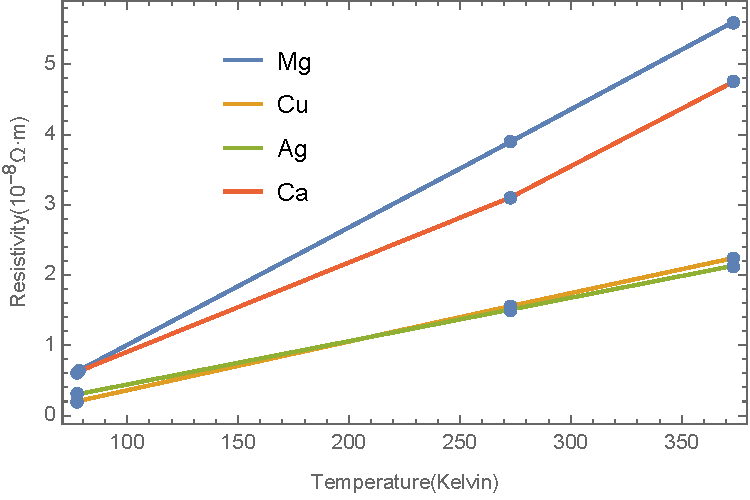
\includegraphics[width=0.6\linewidth]{tau}
	      	\caption{$\rho-T$ of the metals.}
	      	\label{fig:rhoT}
	      \end{figure}

\end{enumerate}

\section*{Problem \RMN{3}}
Plasma frequency $\omega_p$ is given by
\begin{equation}
	\omega_p^2 = \frac{n e^2}{m\varepsilon_0}
\end{equation}
in SI unit system.

For \ce{Ag} and \ce{Au}, their plasma frequencies are
\begin{align}
	\ce{Ag}\!: \omega_p & = \SI{1.364e16}{\radian\per\second} , \\
	\ce{Au}\!: \omega_p & = \SI{1.370e16}{\radian\per\second},
\end{align}
here we suppose ion charge $Z$ of \ce{Au} is $1$.
The maximum frequency of light in the visible range is
\begin{equation}
	\begin{split}
		\omega_\text{max} &= \frac{2\pi c}{\lambda}\\
		&= \frac{2\pi \times \SI{3e8}{\meter \radian\per\second}}{\SI{4000}{\angstrom}} \\
		&=  \SI{4.71e15}{\radian\per\second}.
	\end{split}
\end{equation}
So these two metals display identical mirror-like properties.
And both the plasma frequencies of \ce{Ag} and \ce{Au} are greater than $\omega_\text{max}$.
So they are out of the range of visible light. Therefore it is not consistent.

\section*{Problem \RMN{4}}
Let $\bm{p}(t) = \bm{p}(\omega) \ee^{-\ii \omega t}$, substitute into
\begin{equation}
	\frac{d\bm{p}(t)}{dt} + \frac{\bm{p}(t)}{\tau} = - e (\bm{E} + \frac{\bm{v}}{c }\times \bm{H}),
\end{equation}
we have
\begin{align}
	\Big(- \ii \omega + \frac{1}{\tau}\Big) p_x (\omega ) & = - e E_x -\omega_c p_y(\omega), \\
	\Big(- \ii \omega + \frac{1}{\tau}\Big) p_y (\omega ) & = - e E_y +\omega_c p_x(\omega).
\end{align}
Multiply $\left( -\frac{ne}{m}\right) $ on both sides, and with $-\frac{nep}{m}=j$ we have
\begin{align}
	j_x  \Big(- \ii \omega + \frac{1}{\tau}\Big) & = \frac{ne^2}{m} E_x - \omega_c j_y, \label{eq:jx} \\
	j_y  \Big(- \ii \omega + \frac{1}{\tau}\Big) & = \frac{ne^2}{m} E_y + \omega_c j_x. \label{eq:jy}
\end{align}
Substitute \eqref{eq:jy} into \eqref{eq:jx}, we have
\begin{align}
	j_x & = \frac{ne^2}{m} \frac{\frac{1}{\tau}-\ii \omega}{\big(\frac{1}{\tau} - \ii \omega\big)^2 + \omega_c^2 } E_x - \frac{ne^2}{m}\frac{\omega_c}{\big(\frac{1}{\tau} -\ii \omega\big)^2 + \omega_c^2 }E_y, \\
	j_y & = \frac{ne^2}{m} \frac{\omega_c}{\big(\frac{1}{\tau} -
	\ii\omega\big)^2 + \omega_c^2 }E_x + \frac{ne^2}{m} \frac{ \frac{
	1}{\tau}-\ii \omega}{\big(\frac{1}{\tau} - \ii \omega\big)^2 +
	\omega_c^2} E_y.
\end{align}
It is obvious that $\sigma_{xx} = \sigma_{yy}$, and $\sigma_{xy} = - \sigma_{yx}$.
Now let's prove
\begin{align}
	\sigma_{xx} & = \frac{ne^2}{m} \frac{\frac{1}{\tau}-\ii \omega}{\big(\frac{1}{\tau} - \ii \omega\big)^2 + \omega_c^2 }, \\
	\sigma_{xy} & =  - \frac{ne^2}{m}\frac{\omega_c}{\big(\frac{1}{\tau} -\ii \omega\big)^2 + \omega_c^2 }.
\end{align}
First consider
\begin{equation}
	\begin{split}
		\frac{\frac{1}{\tau}-\ii \omega}{\big(\frac{1}{\tau} - \ii \omega\big)^2 + \omega_c^2 } &= \frac{1- \ii \omega \tau}{\frac{1 - \omega^2\tau^2 - 2\ii \omega\tau + \omega_c^2\tau^2}{\tau}} \\
		&= \frac{(1 -\ii \omega\tau)\tau}{1- \omega^2\tau^2 - 2\ii \omega\tau},
	\end{split}
\end{equation}
here it is due to $\omega \gg \omega_c$, thus $\omega^2\tau^2 \gg \omega_c^2\tau^2$.
Then
\begin{equation}
	\begin{split}
		\frac{(1 -\ii \omega\tau)\tau}{1- \omega^2\tau^2 - 2\ii \omega\tau} &=
		\frac{\tau (1-\ii \omega\tau)\big[ (1 - \omega^2\tau^2) + 2\ii \omega\tau \big] }{\big[ (1 - \omega^2\tau^2) - 2\ii \omega\tau \big]\big[ (1 - \omega^2\tau^2) + 2\ii \omega\tau \big] } \\
		&= \tau \frac{1+\omega^2\tau^2 + \ii\omega\tau + \ii \omega^3\tau^3}{1+\omega^4\tau^4+2\omega^2\tau^2 }\\
		&= \tau \Big( \frac{1+\omega^2\tau^2}{1+\omega^4\tau^4+2\omega^2\tau^2 }
		+ \frac{ \ii\omega\tau + \ii \omega^3\tau^3}{1+\omega^4\tau^4+2\omega^2\tau^2 }\Big)\\
		&= \tau \bigg( \Big(\frac{1}{1+\omega^2\tau^2}\Big)^2 +  \frac{\ii\omega\tau}{1+\omega^2\tau^2}\bigg) \\
		&\approx \tau \bigg(0 + \frac{\ii\omega\tau}{1+\omega^2\tau^2}\bigg)\\
		&= \frac{\ii\omega\tau^2}{1+\omega^2\tau^2} \\
		&\approx  \frac{\ii\omega\tau^2}{\omega^2\tau^2}\\
		&= \frac{\ii}{\omega},
	\end{split}
\end{equation}
here we used $\omega\tau \gg 1$ for twice.
Thus
\begin{equation}
	\begin{split}
		\frac{ne^2}{m} \frac{\frac{1}{\tau}-\ii \omega}{\big(\frac{1}{\tau} - \ii \omega\big)^2 + \omega_c^2 } &= \frac{ne^2}{m }\frac{\ii}{\omega} \\
		&= \frac{\ii\omega_p^2}{4\pi\omega }.
	\end{split}
\end{equation}
Now let's prove $\sigma_{xy} = \frac{\omega_c\omega_p^2}{4\pi\omega^2 }$.
First consider
\begin{equation}
	\begin{split}
		\frac{\omega_c}{\big(\frac{1}{\tau} -\ii \omega\big)^2 + \omega_c^2 } &= \sigma_{xx} \times \Big( -
		\frac{\omega_c}{\frac{1}{\tau} -\ii\omega } \Big)\\
		&= \frac{-\omega_c \tau -\ii \omega_c\omega\tau^2}{1+\omega^2\tau^2}\sigma_{xx}\\
		&= \Big( -\frac{\omega_c}{\omega^2\tau } - \frac{\ii \omega_c}{\omega }\Big)\sigma_{xx}\\
		&=  \frac{\ii\omega_c}{\omega }\frac{\ii \omega_p^2}{4\pi\omega } \\
		&=  \frac{\omega_c\omega_p^2}{4\pi\omega^2 } =\sigma_{xy}.
	\end{split}
\end{equation}
Here we used $\omega^2\tau^2 \gg 1$, and $\frac{\omega_c}{\omega}\frac{1}{\omega\tau} = 0$.



\section*{Problem \RMN{5}}
With static field, we have
\begin{align}
	\frac{p_x}{\tau} & = -e E_x - \omega_c p_y, \\
	\frac{p_y}{\tau} & = -e E_y + \omega_c p_x, \\
	\frac{p_z}{\tau} & = -e E_z.
\end{align}
By $j=-\frac{nep}{m}$, we have
\begin{align}
	\frac{j_x}{\tau} & = \frac{ne^2}{m}E_x - \omega_c j_y,\label{eq:jxt} \\
	\frac{j_y}{\tau} & = \frac{ne^2}{m}E_y + \omega_c j_x,\label{eq:jyt} \\
	\frac{j_z}{\tau} & = \frac{ne^2}{m}E_z.
\end{align}
By substitute \eqref{eq:jxt} into \eqref{eq:jyt}, we have
\begin{align}
	j_x & = \frac{ne^2\tau}{m}\frac{1}{1+(\omega_c\tau)^2}(E_x - \omega_c\tau E_y), \\
	j_y & =\frac{ne^2\tau}{m}\frac{1}{1+(\omega_c\tau)^2}(\omega_c\tau E_x + E_y),  \\
	j_z & = \frac{ne^2\tau}{m}E_z.
\end{align}
Therefore the matrix can be written as
\begin{equation}
	\sigma = \frac{\sigma_0}{1+(\omega\tau)^2}
	\begin{pmatrix}
		1            & -\omega_c\tau & 0                  \\
		\omega_c\tau & 1             & 0                  \\
		0            & 0             & 1+(\omega_c\tau)^2
	\end{pmatrix}.
\end{equation}
Here $\sigma_{yx}=\frac{\sigma_0}{1+(\omega_c\tau)^2}\omega_c\tau$, if $\omega_c\tau\gg1$, then
\begin{equation}
	\begin{split}
		\sigma_{yx} &= \frac{\sigma_0\omega_c\tau}{1+(\omega_c\tau)^2}\\
		&= \frac{\sigma_0}{\omega_c\tau}\\
		&= \frac{\frac{ne^2\tau}{m}}{\frac{eH\tau}{mc}}\\
		&= \frac{nec}{H} = -\sigma_{xy}.
	\end{split}
\end{equation}
Here $\sigma_{xx} = \frac{\sigma_0}{1+(\omega_c\tau)^2} = \frac{ne^2\tau}{m}\frac{1}{(\omega_c\tau)^2} \approx 0$.
The inverse matrix of $\sigma$ is
\begin{equation}
	\rho = \sigma^{-1} = \begin{pmatrix}
	\frac{1}{\sigma_0} & \frac{\omega_c\tau}{\sigma_0} & 0\\
	-\frac{\omega_c\tau}{\sigma_0} & \frac{1}{\sigma_0} & 0\\
	0 & 0 & \frac{1}{\sigma_0}
	\end{pmatrix}.
\end{equation}
That is to say, $\bm{E} = \rho\bm{J}$.
Hall resistivity is $\frac{E_y}{j_x}$, thus is $ -\frac{\omega_c\tau}{\sigma_0} = -\frac{H}{nec}$, so Hall conductivity is
$-\frac{nec}{H} = \sigma_{xy}$.

\bibliographystyle{unsrt}
\bibliography{ref}
\end{document}
